% This is for chapter 3
\chapter{The ROC Surface of Modified Extended Neyman Pearson Test}
Previous chapter showed the MENP framework could achieve the largest probability of detection under any possible probability of false alarm constraints. This chapter proposes the Receiver of Characters surface of MENP test (M-ROC) to depict the relationship between probability of detection and probability of false alarm constraints under MENP framework. Three examples,  concerning the Gaussian case and Chi-Square case, will be presented after that. An analysis of the relationship between the probability of detection and the probability of false alarm constraints will be performed. 

\section{Modified Receiver of Characters of MENP test}

The ROC surface of MENP test (M-ROC) depicts the relationship between $P_d$ and $c_1, c_2, ..., c_M$. On one hand, it  illustrates the largest $P_d$ can be achieved under the constraint $\mathbf{P}_{f} \leq \mathbf{c}$, on the other hand, it provides the range of $\mathbf{c}$ for a given $P_d$.
Points $(P_d, c_1, c_2, ..., c_M)$ on M-ROC  surface can be divided into two types: 
\\1. Those with $[c_1, c_2, ..., c_M] \in \alpha^+$. Define this set of points as $M_0$; 
\\2. Those with $[c_1, c_2, ..., c_M] \notin \alpha^+$. Define this set of points as $M_1$. 

Obviously points in $M_0$ can be achieved by MENP (\rmnum{1}) and points in $M_1$ can  be achieved by MENP (\rmnum{2}). Next we consider a property of M-ROC surface.

\noindent \textbf{Property 1}
\noindent \textit{
  \noindent Assume hypotheses given as:
}
\begin{equation}
\begin{split}
H_0:\;\;\;\;\;\;&X \sim f_0(x)\\
H_1:\;\;\;\;\;\;&X \sim f_1(x)\\
  &......\\
H_M:\;\;\;\;\;\;&X \sim f_M(x)
\end{split}
\end{equation}
\textit{
  define $g(x) = \frac{\sum_{i=1}^{M}k_if_i(x)}{f_0(x)}$ and let $F_i(x)$ represent the CDF of hypothesis $H_i$ ($i = 1, ..., M$). If $g(x)$ is a monotonically increasing function of $x$ for any non-negative $k_i\;\;(i = 1, ..., M)$ and $F_i(x)$ is monotonically increasing function, then we have:}
  
\textit{(1)The region achieved by ENP test with non-negative parameters degenerates to a curve.}

\textit{(2)For a specific false alarm constraints $P_{f_i} \leq c_i\;\;(i = 1, ..., M)$, the decision rule for MENP test is $x \substack{\bar{H}_0 \\ \geq \\ < \\H_0} x_0$, where $x_0 = \min(F_1^{-1}(c_1), ..., F_M^{-1}(c_M))$.}

\textit{(3)The expression of $P_d$, $P_{f_1}$, ..., $P_{f_M}$ can be written as}
\begin{equation}
\label{equ: chi pd}
  \begin{split}
    P_d & = F_0(x_0)\\
        P_{f_1} & = F_1(x_0)\\
        &......\\
            P_{f_M} & = F_M(x_0)
  \end{split}
\end{equation}

\noindent \textbf{PROOF}
According to the definition, $M_0$ is the region achieved by ENP test with $k_i \geq 0 (i=1, ..., M)$. The ENP decision rule is
\begin{equation}
\label{1127a}
\frac{\sum_{i=1}^{M}k_if_i(x)}{f_0(x)} \substack{\bar{H}_0 \\\geq\\< \\H_0}1\,.
\end{equation}
From the condition $g(x) = \frac{\sum_{i=1}^{M}k_if_i(x)}{f_0(x)} $, \eqref{1127a} can be written as 
\begin{equation}
\label{dec: gx}
g(x)\substack{\bar{H}_0 \\\geq\\< \\H_0}1
\end{equation}
Since $g(x)$ is a monotonically increasing function with $x$, hence $g^{-1}(x)$ exists and \eqref{dec: gx} can be written in form of 
\begin{equation}
\label{dec: x0}
x\substack{\bar{H}_0 \\\geq\\< \\H_0}x_0\,,
\end{equation}
where $x_0 = g^{-1}(1)$.
Under decision rule \eqref{dec: x0}, the expression of $P_d$, $P_{f_1}$, ..., $P_{f_M}$ can be written in form of: 
\begin{equation}
\begin{split}
\label{equ: pd under x0}
P_d &= \text{Pr}(X \leq x_0 | H_0) = F_0(x_0)\\
P_{f_1} &= \text{Pr}(X \leq x_0 | H_1) = F_1(x_0)\\
  &......\\
P_{f_M} &= \text{Pr}(X \leq x_0 | H_M) = F_M(x_0)
\end{split}
\end{equation}
where $F_0$, $F_1$, ..., $F_M$ are the CDFs of $X$ under $H_0$, $H_1$, ..., $H_M$. From \eqref{equ: pd under x0}, $P_{f_1}$ determines $x_0$ that in turn determines $P_{f_2}$, ..., $P_{f_M}$, $P_d$. Hence for a given $P_{f_1}$, there is only one corresponding $P_{f_i} (i= 1, ..., M)$. Hence the ROC surface with $k_i \geq 0 (i = 1, ..., M)$ degenerates to a curve in this case.

Furthermore, \eqref{dec: x0}  implies for an ENP decision rule with non-negative parameters, there exists an $x_0$ such that the ENP decision rule can be written in form of 
\begin{equation}
\label{1125 dec: x0}
x\substack{\bar{H}_0 \\\geq\\< \\H_0}x_0\,.
\end{equation}

Next we consider the theoretical decision rule $\delta^\ast$ of
\begin{equation}
\begin{split}
\max\;\;\;\; &P_d\\
\text{s.t.}\;\;\;\;&\mathbf{P}_f \leq \mathbf{c}\,,
\end{split}
\end{equation}
where $\mathbf{c} \in (0, 1)$.
From \textbf{Lemma 1} we know $\delta^\ast$ is an ENP test with non-negative parameters. From previous discussion it can be seen there exists an $x_0$ such that $\delta^\ast$ can be written in form of 
\begin{equation}
\label{1124a1}
x\substack{\bar{H}_0 \\\geq\\< \\H_0}x_0\,,
\end{equation}
and the expression of $P_d$ and $\mathbf{P}_f$ are given in \eqref{equ: pd under x0}. 
In the following, we will determine the value of $x_0$. 
As $P_d$ is an increasing function with respect to $x_0$, in order to acquire the maximum $P_d$ we need to achieve the largest $x_0$ while keeping 
\begin{equation}
P_{f_i} \leq c_i\;\;\;\;(i = 1, 2, ..., M)\,.
\end{equation}
Substitute \eqref{equ: pd under x0} into above equation, we have
\begin{equation}
F_i(x_0) \leq c_i (i=1, 2, ..., M)\,.
\end{equation}
\begin{equation}
\label{1125a1}
\therefore\;\;\;\; x_0 \leq F^{-1}_{i}(c_i) \;\;\;\;(i=1, 2, ..., M)\,.
\end{equation}
\eqref{1125a1} can be fulfilled if $x_0$ is 
 smaller or equal to the minimum of $F^{-1}_{i}(c_i)$ ($i=1, 2, ..., M$). This implies the largest $x_0$ can be achieved is $\min(F_1^{-1}(c_1), F_2^{-1}(c_2), ..., F_M^{-1}(c_M))$, i.e.
\begin{equation}
x_0 = \min(F_1^{-1}(c_1), F_2^{-1}(c_2), ..., F_M^{-1}(c_M))\,.
\end{equation}
By using decision rule $\delta^\ast$, we have
\begin{equation}
\begin{split}
\label{equ: pd under x00}
P_d &=  F_0(x_0)\\
P_{f_1} &=  F_1(x_0)\\
  &......\\
P_{f_M} &= F_M(x_0)
\end{split}
\end{equation}
%==================================================================================================
\typeout{}
%region achieved by the ENP test is a curve/ The Gaussian Case
\section{The M-ROC Surface  under Gaussian Hypotheses}
In the following we present two examples, for computing the M-ROC for Gaussian Hypotheses. 

\noindent \textbf{Example 1:}

Assume three hypotheses given as:
\begin{equation}
\label{equ: Gaussian Hypothesis}
\begin{split}
	H_0:\;\;\;\;\;\;\;\;&X \sim \mathcal{N}(-1,1)\\
    H_1:\;\;\;\;\;\;\;\;&X \sim \mathcal{N}(0,1)\\
    H_2:\;\;\;\;\;\;\;\;&X \sim \mathcal{N}(1,10)\,,
\end{split}
\end{equation}
where $\mathcal{N}(\mu,\sigma^2)$ denotes a Gaussian PDF with mean $\mu$ and variance $\sigma^2$.
To form the M-ROC surface, we first consider points that belong to $M_0$.
From section 3.1, we can see that when $(P_d, c_1, c_2) \in M_0$, there exists non-negative $\mathbf{k}$ such that by using decision rule 
\begin{equation}
f_0(x) \substack{H_0 \\ \geq \\ < \\ \bar{H}_0} k_1f_1(x) + k_2f_2(x)
\end{equation}
we have 
\begin{equation}
\begin{split}
\label{1125c0}
&P_d = \int_{-\infty}^{\infty} u(f_0(x) - \sum_{j=1}^{2}k_jf_j(x)) f_0(x)\mathrm{d}x    \,, \\
&P_{f_i} = \int_{-\infty}^{\infty} u(f_0(x) - \sum_{j=1}^{2}k_jf_j(x)) f_i(x) \mathrm{d}x = c_i\;\;\;\;\;    i=1, 2\,.
\end{split}
\end{equation}
We use Matlab to compute the M-ROC for region $M_0$. The values of $k_1$ and $k_2$ range from $0$ to $100$ in steps of $0.01$. Substituting the value of $k_1$ and $k_2$ into \eqref{1125c0}, results in the corresponding $P_d$ $P_{f_1}$ and $P_{f_2}$.  The set $M_0$ is illustrated in Figure \ref{pic: surface for m0 gaussian}. 
From the definition of $M_0$, we know its projection on the $c_1-c_2$ plane is $\alpha^+$.  
 The set $\alpha^+$ for this example is presented in Figure \ref{pic: contour for m0 gaussian}. 

\begin{figure}[!t]
\centering
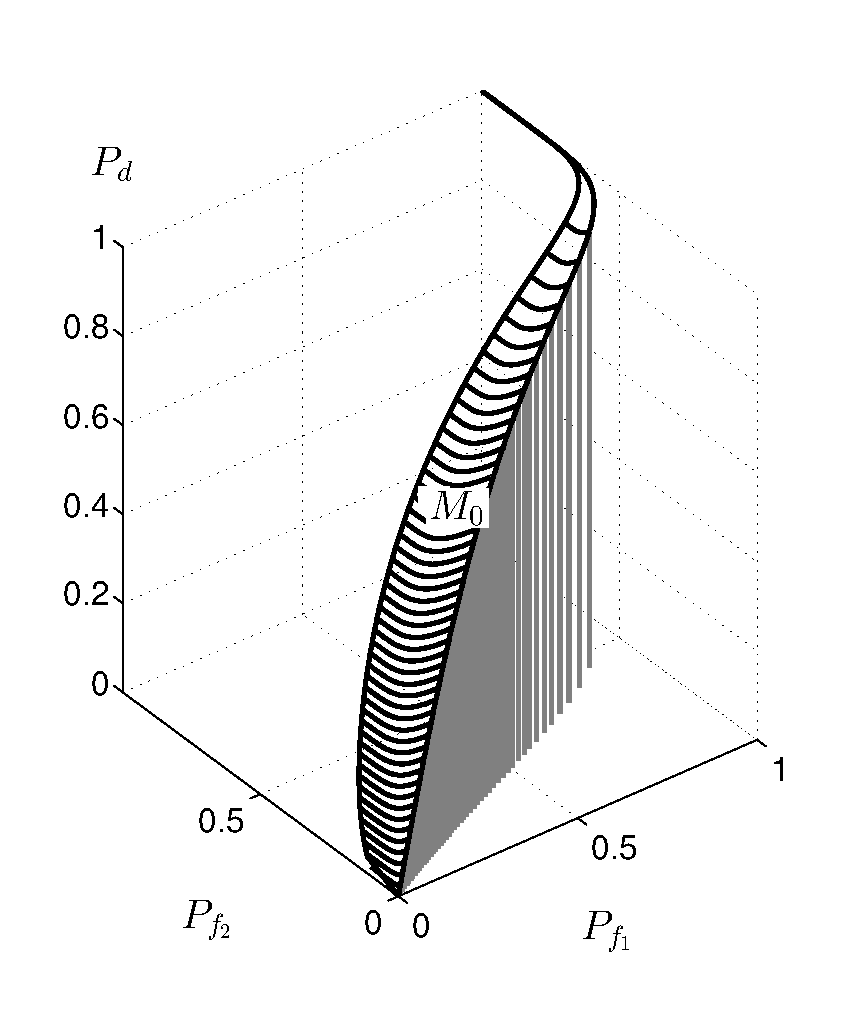
\includegraphics[width=12cm, height=16cm]{3/singleROC.eps}
\caption{Region that can be achieved by Neyman Pearson testing with $k_i \geq 0 (i=1, ..., M)$.}
\label{pic: surface for m0 gaussian}
\end{figure}

\begin{figure}[!t]
\centering
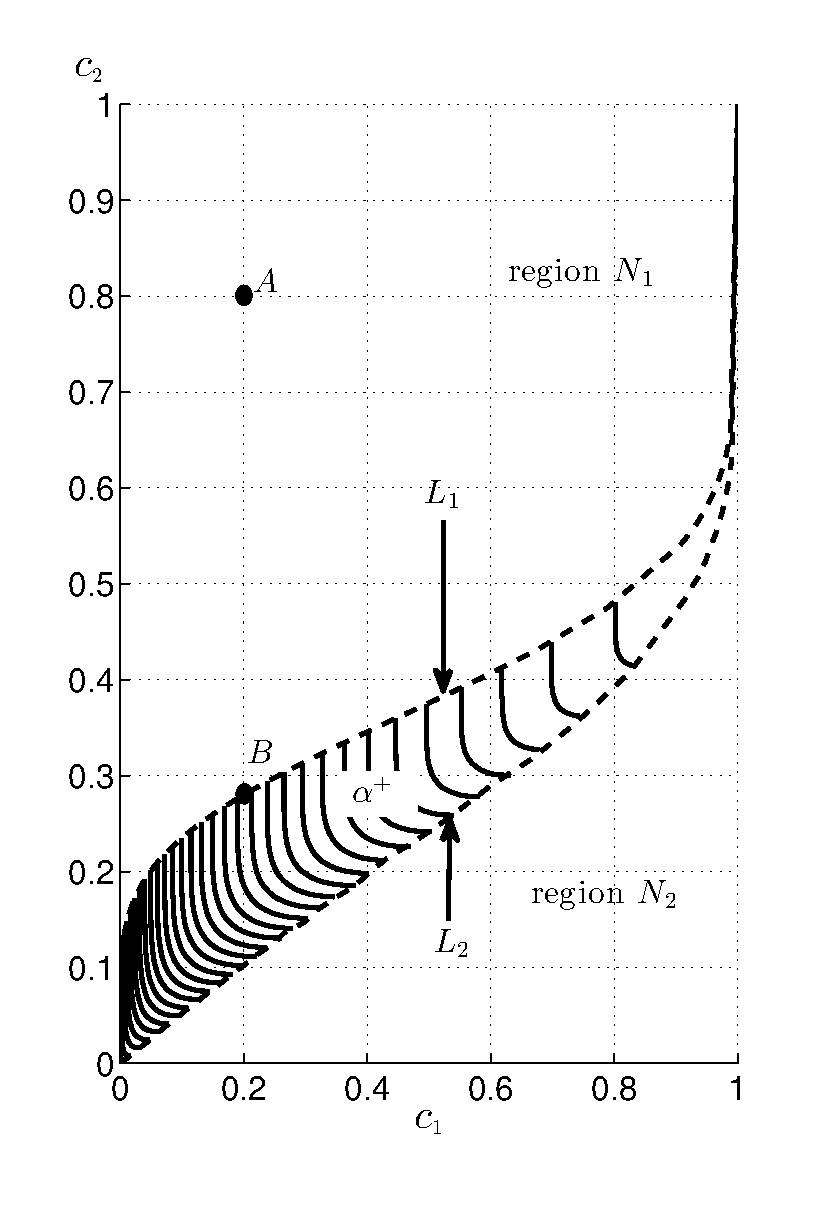
\includegraphics[width=12cm, height = 16cm]{3/singlecontour.eps}
\caption{Region that can be achieved by Neyman Pearson testing with $k_i \geq 0 (i=1, ..., M)$.}
\label{pic: contour for m0 gaussian}
\end{figure}

\begin{figure}[!t]
\centering
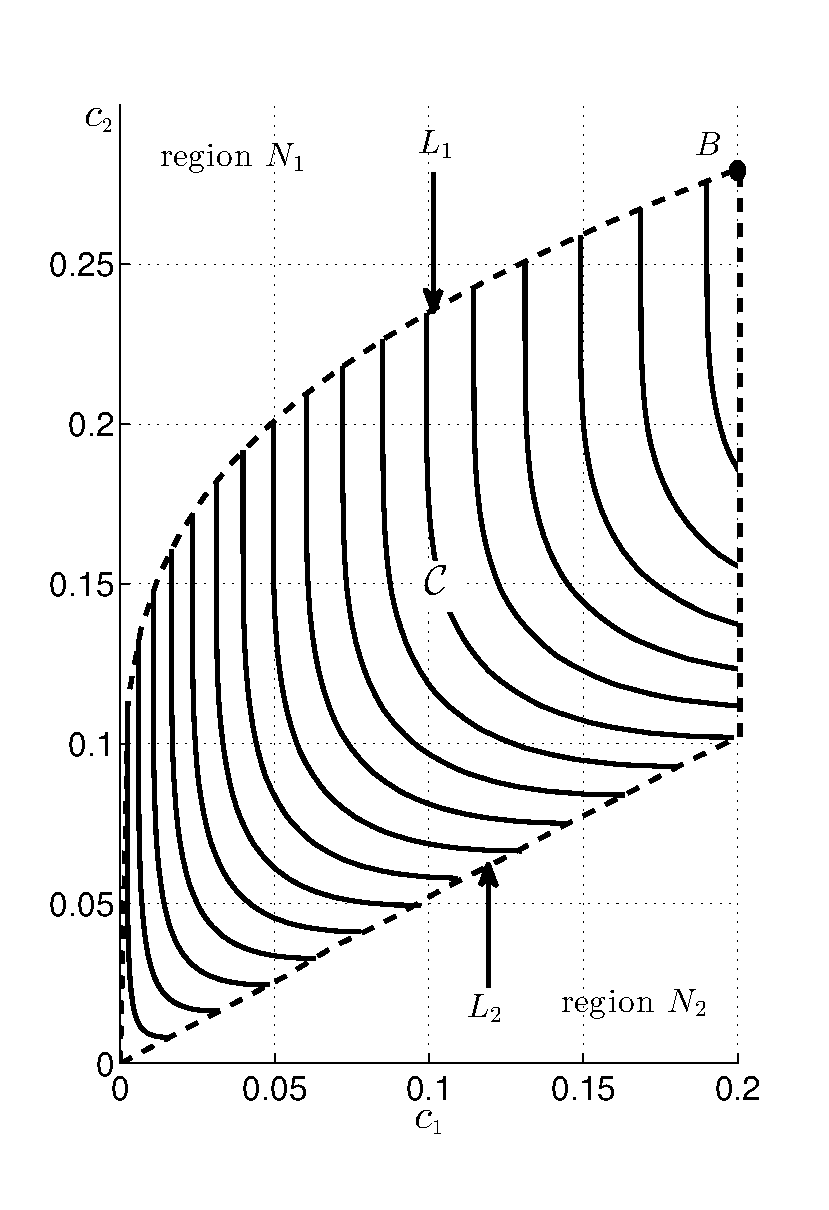
\includegraphics[width=12cm, height = 16cm]{3/singlecontour2.eps}
\caption{The region $\mathcal{C}$ when $c_1 = 0.2$ and $c_2 = 0.8$.}
\label{pic: regionC}
\end{figure}

Define curve $L_1$ as the set of points 
\[
\{ (c_1, c_2) \in L_1 | (c_1, c_2) \in \alpha^+ \;\;\text{and} \;\;(c_1, c_2+\epsilon)\notin \alpha^+ \;\;\;\;\text{for any positive $\epsilon$} \}\,.
\]
Define curve $L_2$ as the set of points 

\[
\{ (c_1, c_2) \in L_2 | (c_1, c_2) \in \alpha^+ \;\;\text{and} \;\;(c_1 + \epsilon, c_2)\notin \alpha^+ \;\;\;\;\text{for any positive $\epsilon$} \}\,.
\]
Let $N_1$ denote the region enclosed by line $c_1 = 0$, $c_2$; line $c_1$, $c_2 = 1$ and curve $L_1$.
Let $N_2$ denote the region enclosed by line $c_1 = 1$, $c_2$; line $c_1$, $c_2 = 0$ and curve $L_2$.
The regions $\alpha^+$, $N_1$ and $N_2$ are shown in Figure \ref{pic: contour for m0 gaussian}.

In the following, we present the decision rule for points belong to regions $N_1$ or $N_2$.

\noindent \textbf{Property 2:}
\textit{\\(1) All points belonging to region $N_1$ or curve $L_1$, if they have the same $c_1$, they have the same decision rule and same $P_d$.
\\(2) All points belonging to region $N_2$ or curve $L_2$, if they have the same $c_2$, they have the same decision rule and same $P_d$.
}

\noindent \textbf{PROOF}
Recall $F(\mathbf{c})$ is defined as the largest $P_d$ that can be achieved under constraint $\mathbf{P}_f = \mathbf{c}$ and 
       $G(\mathbf{c})$ is defined as the largest $P_d$ can be achieved under constraint $\mathbf{P}_f \leq \mathbf{c}$.
Firstly we will show $F(\mathbf{c}) = G(\mathbf{c}) $ when $\mathbf{c} \in \alpha^+$.

According to the definition of $\alpha^+$, for a point $(c_1, c_2) \in \alpha^+$, there exists a decision rule 
\[
\delta:\;\;\;\;f_0(x) \substack{H_0 \\ \geq \\ < \\ \bar{H}_0} k_1f_1(x) + k_2f_2(x) \;\;\;\;(k_1, k_2 \geq 0)
\]
such that under decision rule $\delta$, we have 
\begin{equation}
\label{1125a3}
\mathbf{P}_{f}(\delta) = \mathbf{c}\,.
\end{equation}
From ENP Lemma (\rmnum{2}), we know 
\begin{equation}
\label{1125c1}
P_d(\delta) = F(\mathbf{c})\,.
\end{equation}
Since $k_1, k_2 \geq 0$, according to ENP Lemma (\rmnum{3}), $\delta$ also achieve the largest $P_d$ while keeping $\mathbf{P}_f \leq \mathbf{c}$, i.e. 
\begin{equation}
 P_d(\delta) =G(\mathbf{c}) 
\label{1125a2}
\end{equation}
From \eqref{1125c1} and \eqref{1125a2} we can see $F(\mathbf{c}) = G(\mathbf{c})$ for $\mathbf{c} \in \alpha^+$.
In Section 2.2.2,  we have shown $G(\mathbf{c})$ is a non-decreasing function for each variable of $\mathbf{c}$, hence it can be concluded that $F(\mathbf{c})$ is a non-decreasing function for each variable of $\mathbf{c}$ on set $\alpha^+$.

As it is shown in Figure \ref{pic: contour for m0 gaussian}, A is a point in region ${N}_1$ with coordinates $(c_1, c_2) = (c_{1_A}, c_{2_A})$. In the following we will derive its optimal decision rule through MENP test. By optimal decision rule, we mean   it achieves the largest $P_d$ while keeping $\mathbf{P}_f \leq \mathbf{c}$.  
As point A does not belong to $\alpha^+$, we should use MNEP (\rmnum{2}) to get its decision rule. To do it, the first step is to determine set $\mathcal{C}$, which is the intersection of $\mathcal{A}_c$ and $\alpha^+$. In this case, set $\mathcal{C}$ is plotted in Figure \ref{pic: regionC}.
After we have $\mathcal{C}$, we need to find $\mathbf{c}^0 \in \mathcal{C}$ such that it maximum $F(\mathbf{c})$ among all $\mathbf{c} \in \mathcal{C}$.
Figure \ref{pic: contour for m0 gaussian} and Figure \ref{pic: regionC} shows that point B (with coordinate $(c_{1_B}, c_{2_B})$ where $c_{1_B} = c_{1_A}$) has the largest $c_1$ $c_2$ components among all $\mathbf{c} \in \mathcal{C}$. Since $F(\mathbf{c})$ is a non-decreasing function for $c_1$ and $c_2$ on set $\alpha^+$, it is easy to see
\begin{equation}
  \max_{\mathbf{c} \in \mathcal{C}}\;\;\;\;F(\mathbf{c}) = F(c_{1_B}, c_{2_B})\,.
  \label{2015apr30a0}
\end{equation}
 As point B is in set $\mathcal{C}$, there exists decision rule
 \[
\delta^\ast:\;\;\;\;f_0(x) \substack{H_0 \\ \geq \\ < \\ \bar{H}_0} k_1^\ast f_1(x) + k_2^\ast f_2(x) \;\;\;\;(k_1^\ast, k_2^\ast \geq 0)
 \]
 such that under $\delta^\ast$ we have  $P_{f_1}(\delta^\ast) = c_{1_B}$ and  $P_{f_2}(\delta^\ast) = c_{2_B}$. 
 From ENP (\rmnum{3}), it is easy to see $\delta^\ast$ is the optimal decision rule for point B.
 Since point B satisfies \eqref{2015apr30a0}, by using MENP (\rmnum{2}), we know $\delta^\ast$ is also the optimal decision rule for point A. Thus we can see the optimal decision rule for point A and point B are the same. Since point A lies in region $N_1$, point B lies in region $L_1$ and $c_{1_A} = c_{1_B}$, we can conclude for two points respectively belongs to $N_1$ and $L_1$, if they have the same $c_1$ component, they have the same decision rule and same $P_d$. 

Furthermore, we can see as long as A is in region $N_1$ its decision rule only depends on the value of $c_{1}$.  In other words, as long as A is in region $N_1$, with $c_1 = c_{1_A}$ fixed,  when $c_{2}$ changes, its optimal decision rule and $P_d$ remain the same. Hence we can conclude all points belonging to region $N_1$ or curve $L_1$, if they have the same $c_1$, they have the same decision rule and same $P_d$.

In the same way, we can prove: For points belong to region $N_2$ or curve $L_2$, if they have the same $c_2$ value, they have the same decision rule and same $P_d$.

Q.E.D

Since we have computed $P_d$ for $(c_1, c_2) \in N_0$ and curves $L_1$ and $L_2$ belong to $N_0$, we can get $P_d$ for $(c_1, c_2)$ belongs to $N_1$ or $N_2$ through \textbf{Property 2}. M-ROC surface for this example is given in Figure  \ref{pic: LJS}.
The whole M-ROC is divided into three regions ($M_1$, $M_0$ and $M_2$) to simplify our analysis. In region $M_1$, $P_d$ increases if and only if the value of $c_1$ increases, the value of $c_2$ does not affect $P_d$. On the opposite, in region $M_2$, $P_d$ increases if and only if the value of $c_1$ increases, it does not change with $c_2$. In region $M_0$, when one of $c_1$ or $c_2$ increases, $P_d$ will increase. In all these three regions, $P_d$ is non-decreasing with respect to $c_1$ and $c_2$. 

Next we discuss the different between the ENP test and MENP test concerning this example. 
From Figure \ref{pic: surface for m0 gaussian}, we can see the ENP test works only when the given $(c_1, c_2)$ belongs to set $\alpha^+$. For the case when $(c_1, c_2) \notin \alpha^+$, it cannot provide a solution.  However,  from Figure \ref{pic: LJS}, it can be seen by using the MENP test, we can get the decision rule for all $(c_1, c_2)$. 
In other words, the achievable region of the MENP test is larger than that of the ENP test. 
Besides that, we can see when $(c_1, c_2) \in \alpha^+$, the ENP test and the MENP test provides the same $P_d$. This results from the repetition between the two framework.  
\begin{figure}[!t]
\centering
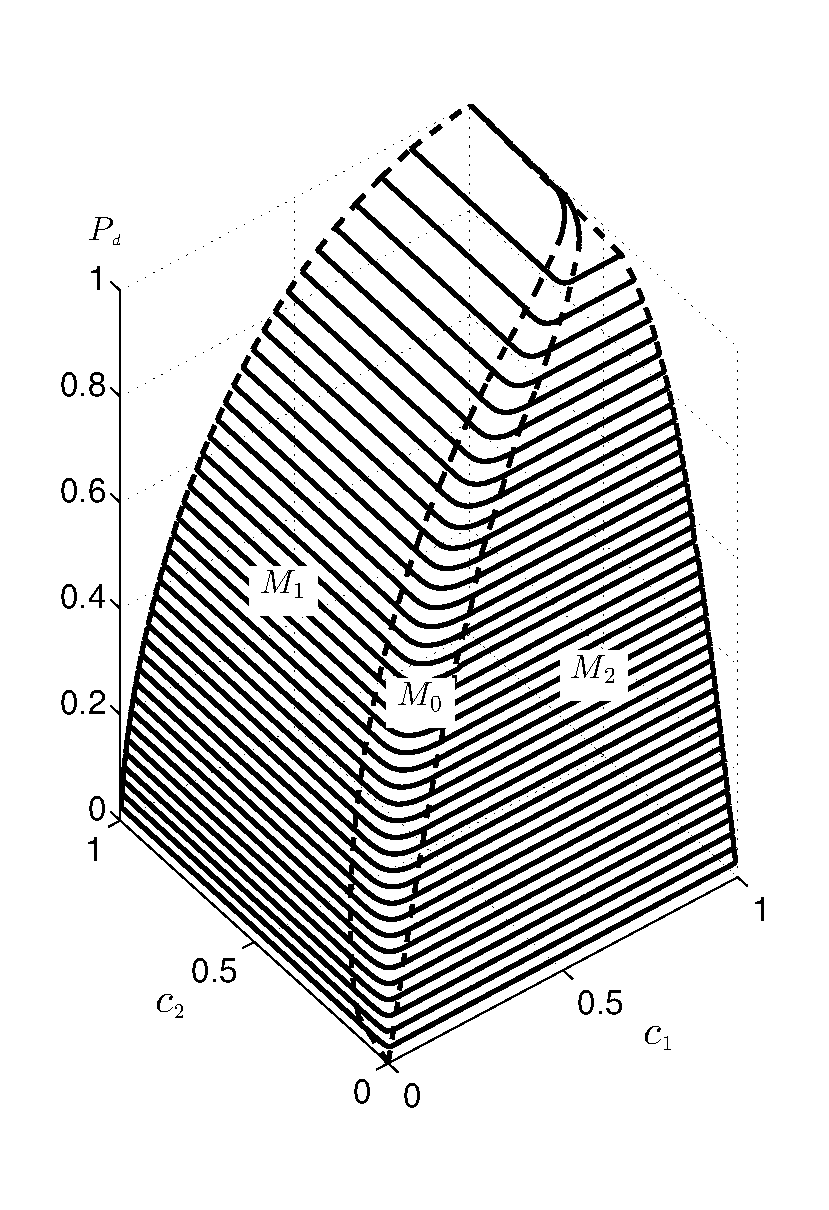
\includegraphics[width=12cm, height=16cm]{3/ROC2.eps}
\caption{The M-ROC surface for Gaussian Hypotheses.}
\label{pic: LJS}
\end{figure}

\noindent \textbf{Example 2:}

Next we consider a more general case of $M+1$ hypotheses given by 
\begin{equation}
\label{equ: m+1 Gaussian Hypo}
\begin{split}
H_0:\;\;\;\;\;\;&X\sim \mathcal{N}(\mu_0, \sigma_0^2)\\
H_1:\;\;\;\;\;\;&X\sim \mathcal{N}(\mu_1, \sigma_1^2)\\
  ......\\
H_M:\;\;\;\;\;\;&X\sim \mathcal{N}(\mu_M, \sigma_M^2)
\end{split}
\end{equation}
We will show when $\sigma_0^2 = \sigma_1^2 = ... = \sigma_M^2$ and $\mu_0 < \mu_i (i = 1, ..., M)$, the region achieved by ENP test with $k_i \geq 0 (i = 1, ..., M)$ degenerates to a curve.

Consider
\begin{equation}
\label{equ: define gx}
g(x) = \sum_{i=1}^{M}k_i\frac{f_i(x)}{f_0(x)}.
\end{equation}
Since 
\begin{equation}
\label{equ: gaussian PDF}
f_i(x) = \frac{1}{\sqrt{2\pi\sigma_i^2}}\exp(-\frac{(x-\mu_i)^2}{2\sigma_i^2}).
\end{equation}
we have
\begin{equation}
\label{g00}
g(x) = \sum_{i=1}^{M}k_i\frac{\frac{1}{\sqrt{2\pi\sigma_i^2}}\exp(-\frac{(x-\mu_i)^2}{2\sigma_i^2})}{\frac{1}{\sqrt{2\pi\sigma_0^2}}\exp(-\frac{(x-\mu_0)^2}{2\sigma_0^2})}
\end{equation}
Substitute  $\sigma_i^2 = \sigma_0^2 (i = 1, ..., M)$ into \eqref{g00}, we have 
\begin{equation}
\label{equ: gx cc}
g(x) = \sum_{i=1}^{M}k_i\exp(\frac{(\mu_i - \mu_0)(2x-\mu_i - \mu_0)}{2\sigma_0^2})
\end{equation}
Defining $p_i = \frac{\mu_i - \mu_0}{2\sigma_0^2}$, \eqref{equ: gx cc} can be written as
\begin{equation}
g(x) = \sum_{i=1}^{M}k_i\exp(p_i(2x-\mu_0 - \mu_i)
\end{equation}
From the condition $\mu_0 < \mu_i (i=1, ..., M)$, we can see $p_i >0$ and  $g(x)$ is a monotonically increasing function with $x$. Here from \textbf{Property 1} we know that $M_0$ (the region achieved by the ENP test with $k_i \geq 0 (i=1, ..., M)$) degenerates to a curve. Moreover, for a specific $\mathbf{c}$, the decision rule is 
\[
x \substack{H_0 \\ \leq \\ > \\ \bar{H}_0} x_0
\]
where $x_0 = \min\{F_1^{-1}(c_1), ..., F_M^{-1}(c_M)\}$. The associated probability of detection is
\[
P_d = F_0(x_0)
\]

Figure \ref{pic: surface for same variance} shows the M-ROC surface for $M=2$, $\mu_0 = 0$, $\mu_1 = 1$, $\mu_2 = 2$ and $\sigma_0^2 = \sigma_1^2 = \sigma_2^2 = 1$. The bold curve is region $M_0$.
To simplify the analysis, the whole M-ROC surface is devided into 3 regions ($M_1$, $M_0$ and $M_2$) as it is shown in Figure \ref{pic: surface for same variance}.  In region $M_1$, $P_d$ increases if and only if the value of $c_1$ increases, the value of $c_2$ does not affect $P_d$. On the opposite, in region $M_2$, $P_d$ increases if and only if the value of $c_1$ increases, it does not change with $c_2$. In region $M_0$, $P_d$ increases if and only if both $c_1$ and $c_2$ increase (This is different from Example 1, because in this case, region $M_0$ degenerates to a curve). 
In all these three regions, $P_d$ is non-decreasing with respect to $c_1$ and $c_2$. 

From the definition of $M_0$, we know $M_0$ is the region can also be achieved by both ENP test and MENP test. We can see, comparing to the ENP test, the MENP test has a much larger achievable region (the MENP test can achieve the $P_d$ for the whole $c_1-c_2$ plane, while the ENP test can only achieve the $P_d$ when $(c_1, c_2)$ lies in $\alpha^+$, which is also a curve because $\alpha^+$ is the projection of $M_0$). 

\begin{figure}[!t]
\centering
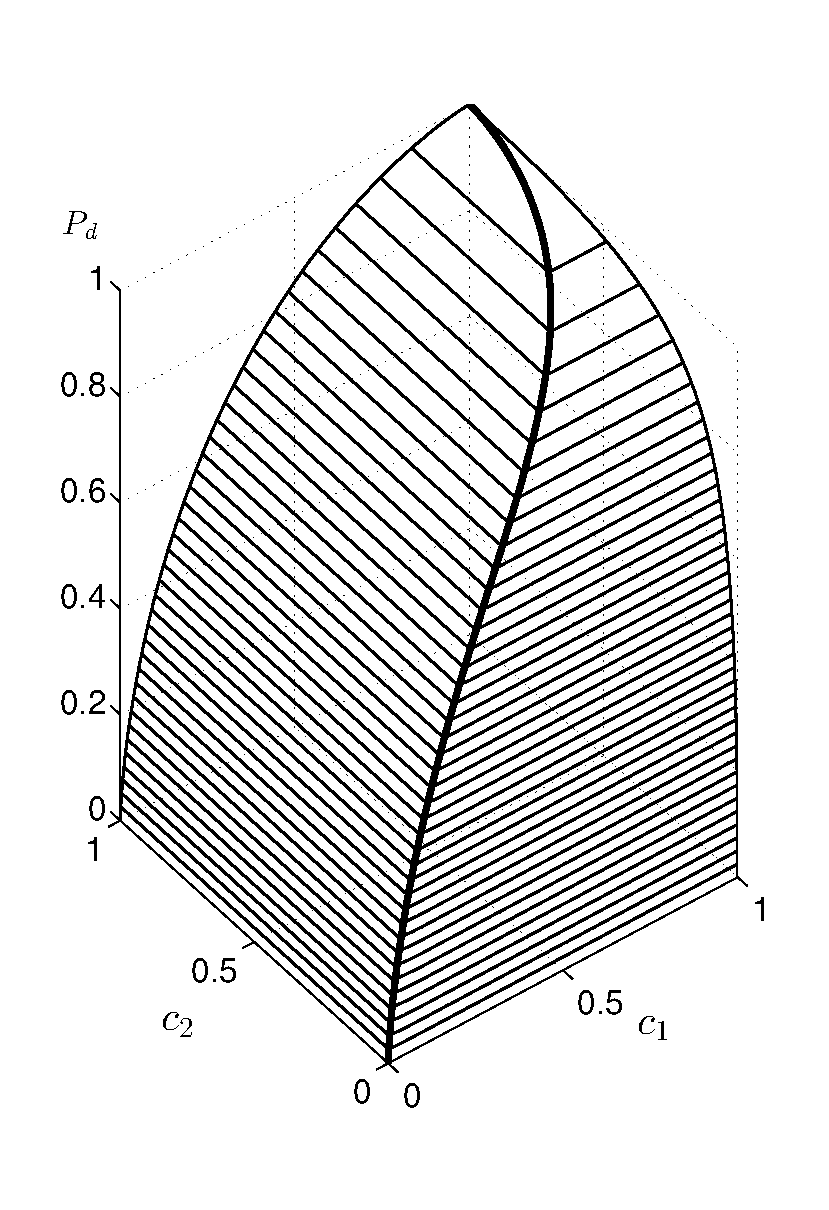
\includegraphics[width=12cm, height=16cm]{3/gaussian.eps}
\caption{The M-ROC for Gaussian distribution with same variance.}
\label{pic: surface for same variance}
\end{figure}


%==================================================================================================
\typeout{}
% Chi-Square Case
\subsection{MROC Surface under Chi-Square Hypotheses}
\noindent\textbf{Example:}

Assume $M+1$ hypotheses  given as:
\begin{equation}
  \label{equ: Chisquare Hypothesis}
  \begin{split}
    H_0:\;\;\;\;\;\;\;\;&\frac{X}{\sigma_0^2} \sim \mathcal{X}^2(2N)\\
    H_1:\;\;\;\;\;\;\;\;&\frac{X}{\sigma_1^2} \sim \mathcal{X}^2(2N)\\
    &......\\
    H_M:\;\;\;\;\;\;\;\;&\frac{X}{\sigma_2^M} \sim \mathcal{X}^2(2N)\,,
  \end{split}
\end{equation}
where $\mathcal{X}^2(2N)$ is the Chi-square distribution with  $2N$ degree freedom($N$ is an integer, $\sigma_0^2 < \sigma_1^2, ..., \sigma_M^2$ and $\sigma_i^2 \neq \sigma_j^2$ if $i \neq j$). By a random variable transformation space \cite{mark2011probability}, we can get the PDFs for the hypotheses:

\def \CHISQU[#1]{\frac{1}{#1 2^N\Gamma(N)}\left(\frac{x}{#1}\right)^{N-1}\exp\left(-\frac{x}{2#1}\right)\\}
\begin{equation}
  \label{equ: Chisquare Distribution}
  \begin{split}
    H_0:\;\;\;\;\;\;\;\;&f_0(x) = \CHISQU[\sigma_0^2]\\
    H_1:\;\;\;\;\;\;\;\;&f_1(x) = \CHISQU[\sigma_1^2]\\
    &......\\
    H_M:\;\;\;\;\;\;\;\;&f_2(x) = \CHISQU[\sigma_M^2]\,.
  \end{split}
\end{equation}

In the following, we will prove that in this example the region achieved by ENP test with $\mathbf{k}$ degenerates to a curve.

Consider
\begin{equation}
\label{equ: decision rule chi}
  g(x) = \frac{\sum_{i=1}^{M}k_if_i(x)}{f_0(x)} \;\;\;\;k_i \geq 0
\end{equation}
Substituting $f_i(x) (i=1, ..., M)$ from \eqref{equ: Chisquare Distribution} into \eqref{equ: decision rule chi}, we get:

\begin{equation}
  \label{equ: decision rule chi 1}
g(x) = \sum_{i=1}^{M}k_i'\exp{(\frac{1}{2\sigma_0^2} - \frac{1}{2\sigma_i^2})x} 
\end{equation}
where $k_i' = k_i(\frac{\sigma_0}{\sigma_i})^{2N}, i= 1, ..., M$. Define $p_i = \frac{1}{2\sigma_0^2} - \frac{1}{2\sigma_i^2}, i=1, ..., M$. Hence $g(x) =  \sum_{i=1}^{M}k_i'\exp{(p_ix)}$.

The parameters $k_i' (i=1, ..., M)$ are always non-negative when $k_i (i=1, ..., M)$ are such, and from 
 the condition $\sigma_0^2 \leq \sigma_i^2 (i=1, ..., M)$ we can conclude $p_i (i=1, ..., M)$ are positive. Hence $g(x)$ is a monotonically increasing function with $x$. From \textbf{Property 1}, we have that the region achieved by ENP test with $k_i (i = 1, ..., M)$ degenerates to a curve. For a specific $\mathbf{c}$, the decision rule is
\begin{equation}
  \label{equ: decision rule chi 2}
  x \substack{\bar{H}_0 \\ \geq \\ < \\ H_0} x_0\,,
\end{equation}
where $x_0 = \min\{F_1^{-1}(c_1), ..., F_M^{-1}(c_M)\}$,
and the corresponding $P_d = F_0(x_0)$. 

Figure \ref{pic: LJS for chisquare} shows the M-ROC surface for $M=2$, $\sigma_0^2 = 1$, $\sigma_1^2 = 1.1$, $\sigma_2^2 = 1.15$ and $N=120$. The bold curve  is the region $M_0$. 

\begin{figure}[!t]
\centering
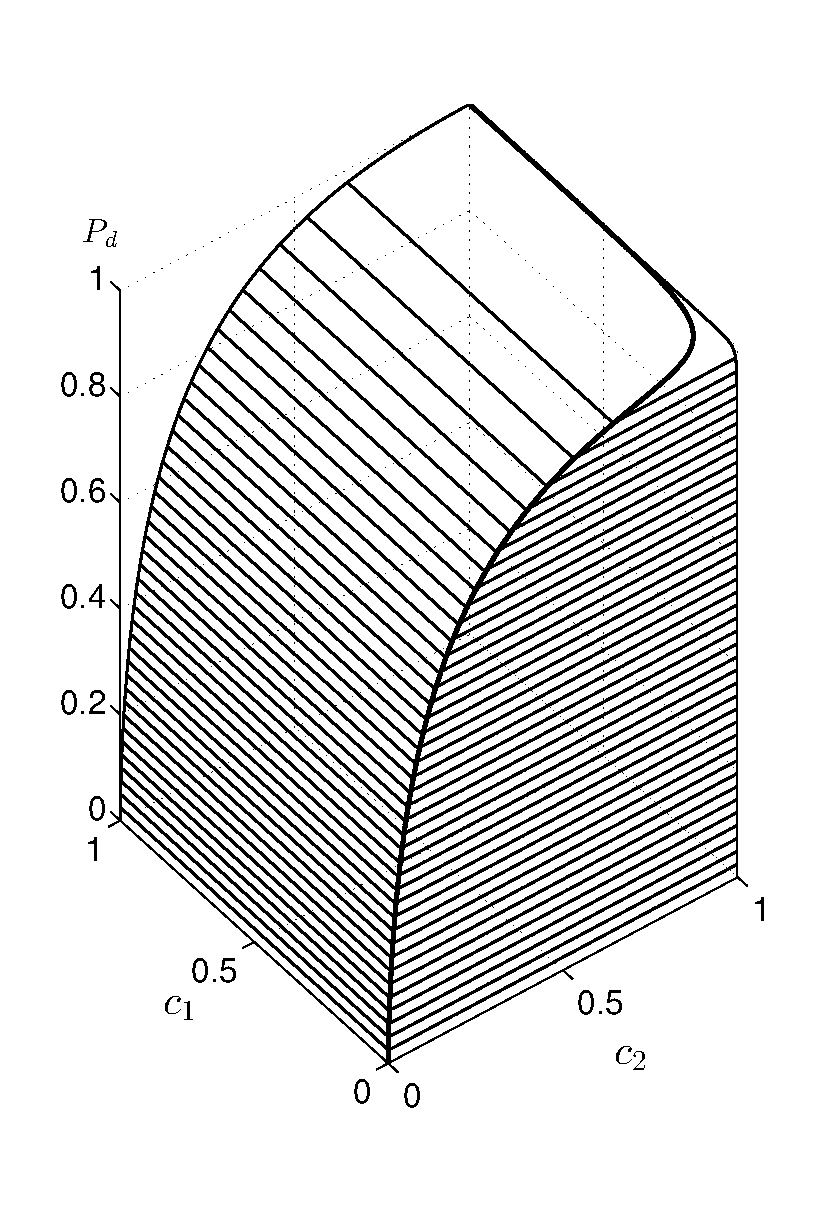
\includegraphics[width=12cm, height=16cm]{3/example3.eps}
\caption{The M-ROC for the Chi-square example.}
\label{pic: LJS for chisquare}
\end{figure}

